\documentclass[tikz,border=2pt]{standalone}
\usepackage{amsmath,amssymb}
\usepackage{tikz}
\usetikzlibrary{arrows.meta}

\begin{document}
% Euler's formula: e^{i theta} is the point of the unit circle at angle theta, with real part
% cos theta and imaginary part sin theta.
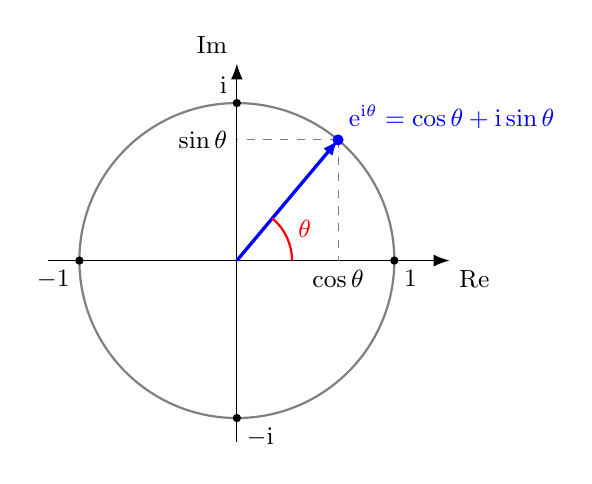
\begin{tikzpicture}[every node/.style={font=\small}, >={Latex[length=2mm]}]
	\draw[->] (-2.4,0) -- (2.7,0) node[below right] {$\mathrm{Re}$};
	\draw[->] (0,-2.3) -- (0,2.5) node[above left] {$\mathrm{Im}$};
	\draw[gray, thick] (0,0) circle (2);
	\draw[dashed, gray] (50:2) -- ({2*cos(50)},0);
	\draw[dashed, gray] (50:2) -- (0,{2*sin(50)});
	\draw[->, blue, very thick] (0,0) -- (50:2) node[above right] {$\mathrm{e}^{\mathrm{i}\theta}=\cos\theta+\mathrm{i}\sin\theta$};
	\fill[blue] (50:2) circle (2pt);
	\draw[red, thick] (0.7,0) arc (0:50:0.7);
	\node[red, font=\small] at (25:0.95) {$\theta$};
	\node[below, font=\small] at ({2*cos(50)},0) {$\cos\theta$};
	\node[left, font=\small] at (0,{2*sin(50)}) {$\sin\theta$};
	\fill (2,0) circle (1.5pt) node[below right] {$1$};
	\fill (0,2) circle (1.5pt) node[above left] {$\mathrm{i}$};
	\fill (-2,0) circle (1.5pt) node[below left] {$-1$};
	\fill (0,-2) circle (1.5pt) node[below right] {$-\mathrm{i}$};
\end{tikzpicture}
\end{document}
